% =====================================================================
%  Online Appendix
%  Anticipation, Not Reaction. Wang and Jin (2026).
% =====================================================================
\documentclass[11pt,a4paper]{article}

\usepackage[utf8]{inputenc}
\usepackage[T1]{fontenc}
\usepackage[margin=2.4cm]{geometry}
\usepackage{setspace}
\onehalfspacing
\usepackage{booktabs}
\usepackage{amsmath,amssymb}
\usepackage{graphicx}
\usepackage{caption}
\usepackage{titlesec}
\usepackage{hyperref}
\PassOptionsToPackage{hyphens}{url}
\usepackage{url}
\usepackage{xurl}
\urlstyle{tt}
\newcommand{\code}[1]{\path{#1}}
\sloppy

\graphicspath{{figures/}}
\hypersetup{hidelinks}
\captionsetup{font=small,labelfont=bf}
\renewcommand{\thesection}{\Alph{section}}
\newcommand{\simk}[1]{\ensuremath{\mathrm{sim}_{#1}}}

\title{\textbf{Online Appendix}\\[3pt]
\large Anticipation, Not Reaction: Media Discourse, FOMC Communication,
and Pre-Announcement Volatility}
\author{Duo (Doris) Wang \quad Yuzhao (Jerry) Jin}
\date{This draft: \today}

\begin{document}
\maketitle

This appendix documents the corpus coverage in full, the remaining identification
output, the computational architecture, and the reproducibility package. Section
and equation references of the form ``main text'' point to the manuscript.

% =====================================================================
\section{Corpus coverage by lag}

Table~\ref{tab:covfull} reports the number of meetings with media coverage at each
lag for the three corpora, extending Table~1 of the main text. The broad corpus
has complete coverage at every lag from $-3$ to $+3$ for the 33 meetings in the
estimation window; the curated outlets have uneven coverage that thins at the
extreme lags. This table is the reproducible basis for the sample restrictions used
throughout the paper: every reported $n$ can be read off it.

\begin{table}[h]
\centering
\caption{Meetings with coverage by source and lag.}
\label{tab:covfull}
\small
\begin{tabular}{rrrr}
\toprule
Lag $k$ & GDELT & Guardian & NYT \\
\midrule
-7 &  & 18 & 6 \\
-6 &  & 19 & 8 \\
-5 &  & 22 & 13 \\
-4 &  & 15 & 6 \\
-3 & 33 & 5 & 10 \\
-2 & 33 & 13 & 12 \\
-1 & 33 & 15 & 12 \\
+0 & 33 & 62 & 21 \\
+1 & 33 & 37 & 22 \\
+2 & 33 & 29 & 22 \\
+3 & 33 & 14 & 8 \\
+4 &  & 14 & 6 \\
+5 &  & 12 & 6 \\
+6 &  & 23 & 7 \\
+7 &  & 20 & 14 \\
\bottomrule
\end{tabular}
\end{table}

\begin{figure}[h]
\centering
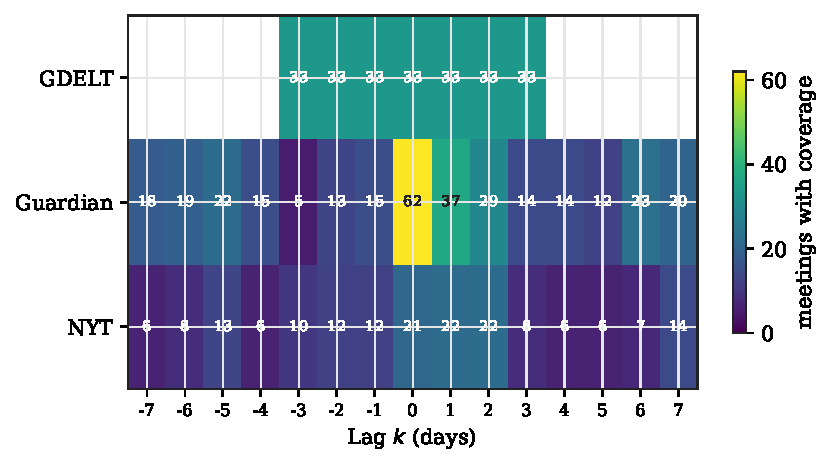
\includegraphics[width=0.7\textwidth]{fig8_coverage.pdf}
\caption{Coverage heatmap. Darker cells indicate more meetings covered at that
source and lag.}
\label{fig:covheat}
\end{figure}

% =====================================================================
\section{Additional identification output}

\subsection{Granger causality}

Table~\ref{tab:granger} gives the full Granger output for the test of whether
pre-meeting similarity precedes post-meeting volatility across the chronologically
ordered meetings. The evidence of temporal precedence is marginal, significant at
the second lag and not at the first, which is why the main text treats the Granger
result as descriptive rather than as evidence of a causal direction.

\begin{table}[h]
\centering
\caption{Granger causality, \simk{-2} to post-meeting volatility.}
\label{tab:granger}
\small
\begin{tabular}{rrrr}
\toprule
Lag & $F$ & df & $p$-value \\
\midrule
1 & 1.244 & (1,29) & 0.2739 \\
2 & 3.510 & (2,26) & 0.0447 \\
3 & 2.425 & (3,23) & 0.0915 \\
\bottomrule
\end{tabular}
\end{table}

\subsection{Vector autoregression}

Table~\ref{tab:irf} reports the impulse response of standardized post-meeting
volatility to a one-standard-deviation shock in standardized pre-meeting
similarity, from a reduced-form VAR(2) on similarity, volatility, and the VIX. The
cumulative response is positive but modest, consistent with the controlled
regression in which the similarity coefficient is small once the VIX is included.

\begin{table}[h]
\centering
\caption{VAR(2) impulse response of volatility to a similarity shock.}
\label{tab:irf}
\small
\begin{tabular}{rr}
\toprule
Horizon (meetings) & Vol. response to sim. shock \\
\midrule
0 & 0.000 \\
1 & 0.005 \\
2 & 0.497 \\
3 & 0.464 \\
4 & 0.293 \\
5 & 0.203 \\
6 & 0.161 \\
\bottomrule
\end{tabular}
\end{table}

\subsection{Scatter of the raw relationship}

Figure~\ref{fig:scatter} plots the bivariate relationship behind column (1) of the
main regression table.

\begin{figure}[h]
\centering
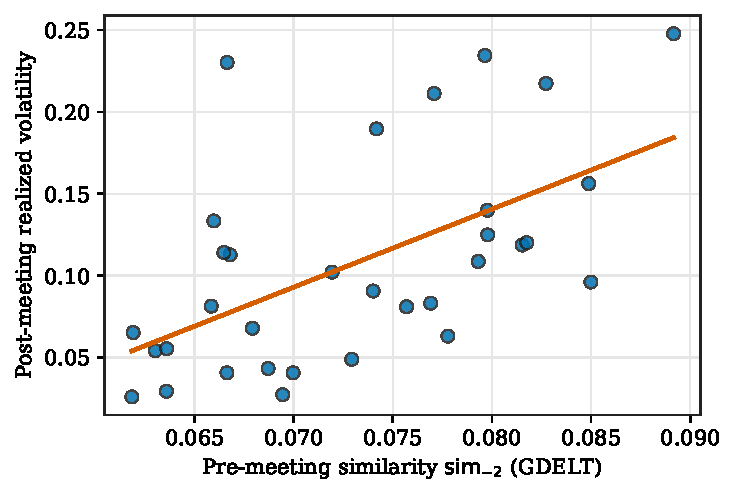
\includegraphics[width=0.55\textwidth]{fig5_scatter_sim_vol.pdf}
\caption{Pre-meeting similarity against post-meeting realized volatility, broad
corpus, with the ordinary-least-squares fit.}
\label{fig:scatter}
\end{figure}

% =====================================================================
\section{Tone measure and timeline}

Figure~\ref{fig:timeline} shows the net tone of the FOMC minutes across the sample,
measured as positive minus negative intensity in the Loughran--McDonald market
dictionary and expressed per thousand tokens. The series reproduces the known
turning points of the decade without any hand labeling: tone falls to its most
negative on the March and April 2020 emergency meetings and drifts steadily more
negative through the 2022--2023 tightening, so the measure is already meaningful
before any market variable is introduced. This is the descriptive basis for the
market-validation result in the main text, where the negative intensity of the same
minutes is shown to move with the pre-meeting VIX and to forecast post-meeting
realized volatility.

\begin{figure}[h]
\centering
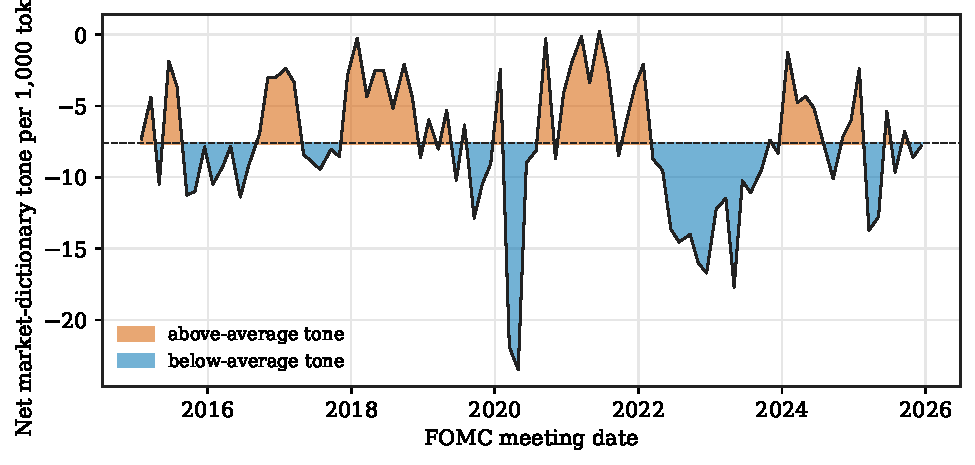
\includegraphics[width=0.8\textwidth]{fig6_hawkish_timeline.pdf}
\caption{Net market-dictionary tone (positive minus negative intensity,
Loughran--McDonald, per 1,000 tokens) across the 88 FOMC minutes, 2015--2025. The
dashed line is the sample mean; shading marks meetings above and below it.}
\label{fig:timeline}
\end{figure}

% =====================================================================
\section{Computational architecture}

The pipeline separates resource-gated stages from the reproducible CPU path.

\paragraph{Distributed stages.} GDELT ingestion reads the Global Knowledge Graph
shards, filters to United States Federal-Reserve-relevant records with Spark SQL,
and writes date-partitioned Parquet
(\code{scripts/ingest/06_spark_ingest_gdelt.py}). Tone scoring broadcasts the
hawkish--dovish lexicon to the executors and applies a grouped pandas
user-defined function (\code{scripts/sentiment/07_spark_sentiment.py}). Cosine
similarity broadcasts the small per-meeting FOMC vectors and keeps the large media
side distributed (\code{scripts/similarity/11_spark_similarity.py}). These
stages run unchanged in a local Spark session for validation on a sample week and
on a five-node cluster for the full corpus.

\paragraph{Resource-gated robustness.} Contextual-embedding similarity with
Sentence-BERT (\code{scripts/similarity/11b_sbert_similarity.py}) and FinBERT
tone (\code{scripts/sentiment/07c_finbert_inference.py}) are implemented and
run on a GPU node; over the full media corpus they are GPU-bound and are therefore
provided as code rather than executed in the CPU package.

\paragraph{Reproducible CPU path.} The panel construction, main regression,
identification battery, tone validation, benchmark, tables, and figures run on a
single node from the committed intermediate artifacts. The workflow is a Snakemake
file with a pinned conda environment and a container image, so the command
\texttt{snakemake -c4 all} regenerates every number and figure in the paper.

\paragraph{Throughput.} The single-node scoring kernel is benchmarked in the main
text (Table~7): the Numba parallel just-in-time implementation is faster than a
pure-Python loop by more than an order of magnitude on a five-million-token
workload, which is what makes full-corpus scoring feasible before the work is
distributed.

% =====================================================================
\section{File-by-file map}

\begin{table}[h]
\centering
\caption{Pipeline scripts.}
\footnotesize
\begin{tabular}{p{6.2cm}p{8.2cm}}
\toprule
Stage & Script \\
\midrule
Panel construction and coverage & \texttt{scripts/analysis/00\_build\_panel.py} \\
Main regression and lead--lag profile & \texttt{scripts/analysis/12\_main\_regression.py} \\
Placebo, Granger, VAR, bootstrap, subsamples & \texttt{scripts/analysis/13\_identification.py} \\
LaTeX tables & \texttt{scripts/analysis/16\_make\_tables.py} \\
Loughran--McDonald tone validation & \texttt{scripts/sentiment/07b\_lm\_dictionary.py} \\
Distributed GDELT ingestion & \texttt{scripts/ingest/06\_spark\_ingest\_gdelt.py} \\
Distributed tone scoring & \texttt{scripts/sentiment/07\_spark\_sentiment.py} \\
Distributed cosine similarity & \texttt{scripts/similarity/11\_spark\_similarity.py} \\
Sentence-BERT similarity (GPU) & \texttt{scripts/similarity/11b\_sbert\_similarity.py} \\
FinBERT tone (GPU) & \texttt{scripts/sentiment/07c\_finbert\_inference.py} \\
Throughput benchmark & \texttt{scripts/benchmark/13\_benchmark.py} \\
Figures & \texttt{scripts/figures/make\_figures.py} \\
\bottomrule
\end{tabular}
\end{table}

\end{document}
